\section[locl]{Intranet Communications}

\subsection{Client-Server Applications and Protocols}

\begin{frame}{Client-Server Applications and Protocols}
	Examples:\pause
	\begin{itemize}[<+->]
		\item \wiki{World Wide Web}{World_Wide_Web} and \wiki{HTTP}{Hypertext_Transfer_Protocol}, \wiki{HTTPS}{HTTPS}
		\item \wiki{Electronic mail}{Email} and \wiki{SMTP}{SMTP}, \wiki{POP3}{Post_Office_Protocol}, \wiki{IMAP}{Internet_Message_Access_Protocol}
	\end{itemize}
	\onslide<4->
	Transport protocols (Layer 4):\pause
	\begin{itemize}[<+->]
		\item Client-Server port numbers
		\item \wiki{TCP}{Transmission_Control_Protocol}, \rfc{791}
		\begin{itemize}
			\item Three-way handshake
			\item Reliable transmission
			\begin{itemize}
				\item Sequence and acknowledge numbers
				\item Checksum and retransmission
			\end{itemize}
			\item Flow control
			\item Congestion control
		\end{itemize}
		\item \wiki{UDP}{User_Datagram_Protocol}, \rfc{768}
		\begin{itemize}
			\item Optional checksum
		\end{itemize}
	\end{itemize}
\end{frame}

\subsection{Dynamic Host Configuration Protocol}

\begin{frame}{Dynamic Host Configuration Protocol}
	\wiki{DHCP}{Dynamic_Host_Configuration_Protocol} (\rfc{2131}), allows automatic configuration of:\pause
	\begin{itemize}[<+->]
		\item IP address
		\item Mask
		\item Default gateway
		\item and more
	\end{itemize}
	\onslide<6->
	Important DHCP Messages\pause
	\begin{itemize}[<+->]
		\item Discover
		\item Offer
		\item Request
		\item Acknowledge
	\end{itemize}
	\onslide<11->
	DHCP uses UDP\pause
	\begin{itemize}[<+->]
		\item Port 68 for client
		\item Port 67 for server
	\end{itemize}
\end{frame}

\begin{frame}{Dynamic Host Configuration Protocol}
	Cisco IOS DHCP Client configuration
	\\\pause\texttt{-if)\#ip address dhcp}
	\\\vspace{0.5cm}\pause Cisco IOS DHCP Server configuration
	\texttt{
		\\\pause \hangindent=2em )\#ip dhcp excluded-address \textit{ip-address [last-ip-address]}
		\\\pause )\#ip dhcp pool \textit{name}
		\\\pause dhcp-)\#network \textit{network-number mask}
		\\\pause dhcp-)\#default-router \textit{address}
		\\\pause dhcp-)\#lease \textit{days [ hours [minutes] ]}
		\\\pause dhcp-)\#dns-server \textit{address}
		\\\pause dhcp-)\#domain-name \textit{domain}
	}\\\vspace{0.5cm}
	\pause Cisco IOS DHCP Relay configuration
	\\\pause\texttt{-if)\#ip helper-address \textit{address}}
\end{frame}
%}

\subsection{Virtual Local Area Networks}

\begin{frame}{VLANs}
	\texttt{
		\begin{columns}
			\begin{column}{0.5\textwidth}
				\begin{tabular}{l}
					\multicolumn{1}{c}{Unmanaged switch}\\
					\hline
					\multicolumn{1}{|c|}{1 2 3 4 5 6 7 8 9 10}\\
					\hline\pause\\
					\#show mac address-table\\
					\hline
					MAC1~~~Fa0/1\\
					MAC2~~~Fa0/2\\
					MAC5~~~Fa0/5\\
					MAC6~~~Fa0/6\\
					\hline
				\end{tabular}
			\end{column}
			\pause
			\begin{column}{0.5\textwidth}
				\begin{tabular}{lll}
					\multicolumn{3}{c}{Switch with VLAN support}\\
					\hline
					\multicolumn{1}{|l}{1 2 3}&\multicolumn{1}{|l}{4 5 6}&\multicolumn{1}{|l|}{7 8 9 10}\\
					\hline\pause\\
					\multicolumn{3}{l}{\#show mac address-table}\\
					\hline
					\multicolumn{3}{l}{VLAN123~~~MAC1~~~Fa0/1}\\
					\multicolumn{3}{l}{VLAN123~~~MAC2~~~Fa0/2}\\
					\hline
					\multicolumn{3}{l}{VLAN456~~~MAC5~~~Fa0/5}\\
					\multicolumn{3}{l}{VLAN456~~~MAC6~~~Fa0/6}\\
					\hline
				\end{tabular}
			\end{column}
		\end{columns}
		\pause\vspace{1cm}
		)\#vlan 2						\hfill	\textcolor<6->{black!50}{Create VLAN}
		\pause\\-vlan)\#name NEW-VLAN	\hfill	\textcolor<7->{black!50}{Rename VLAN}
		\pause\\-vlan)\#interface fa0/3
		\pause\\-if)\#switchport access vlan 3	\hfill	\textcolor<9->{black!50}{Assign VLAN}
		\pause\\\% Access VLAN does not exist. Creating vlan 3
	}
\end{frame}

\begin{frame}{Verifying VLAN and Port Status}
	\texttt{\#show vlan brief
		\pause\\VLAN~Name~~~~~~~Status~~~~Ports
		      \\----~----------~--------- ---------
		      \\1~~~~default~~~~active~~~~Fa0/1, Fa0/2, Fa0/4
		      \\2~~~~NEW-VLAN~~~active
		      \\3~~~~VLAN0003~~~active~~~~Fa0/3
		\vspace{0.5cm}
		\pause\\\#show interface status
		\pause\\Port~~~~~~Name~~~~~~Status~~~~~~~~~~~Vlan 
	          \\Fa0/1~~~~~~~~~~~~~~~connected~~~~~~~~1    
	          \\Fa0/2~~~~~~~~~~~~~~~connected~~~~~~~~1    
	          \\Fa0/3~~~~~~~~~~~~~~~connected~~~~~~~~3
	          \\Fa0/4~~~~~~~~~~~~~~~connected~~~~~~~~1
	}
\end{frame}

\begin{frame}{Access Ports and Trunks}
	\texttt{\framebox[1.1\width]{~frame1~}~~
			\framebox[1.1\width]{~frame2~}~~
			\framebox[1.1\width]{~frame3~} 
			\newline \pause
			\newline                     Fa0/1(1)~~~~Fa0/2(2)~~~~Fa0/3(3)~
			\newline\framebox[1.1\width]{~~~~~~~~~~~Switch~1~~~~~~~~~~~}\pause
			\newline\phantom{            ~~~~~~~~~~~~}Fa0/4(T)\newline\pause
			\newline\phantom{~~~~~~~}\framebox[1.1\width]{~frame1~\only<-7|handout:0>{|~VLAN~1~}}\only<8>{\hfill Native VLAN (802.1Q)}
			\newline\phantom{~~~~~~~}\framebox[1.1\width]{~frame2~|~VLAN~2~}
			\newline\phantom{~~~~~~~}\framebox[1.1\width]{~frame3~|~VLAN~3~} 
			\newline\pause
			\newline\phantom{~~~~~~~~~~~~~}Fa0/4(T)
			\newline\framebox[1.1\width]{~~~~~~~~~~~Switch~2~~~~~~~~~~~}\pause
			\newline                     Fa0/1(1)~~~~Fa0/2(2)~~~~Fa0/3(3)~
			\newline\pause
			\framebox[1.1\width]{~frame1~}~~
			\framebox[1.1\width]{~frame2~}~~
			\framebox[1.1\width]{~frame3~} 
	}
\end{frame}

\begin{frame}{Trunk Encapsulations}
	\wiki{Ethernet Frame}{Ethernet_frame\#Structure}\\\vspace{0.1cm}
	\texttt{%
		\begin{tabular}{|c|c|c|c|c|c|}
			\hline 	6	&6	&2		&46-1500	&4\\
					DM	&SM	&Type	&Data		&FCS\\\hline
		\end{tabular}
	}
	\pause\\\vspace{0.5cm}\wiki{802.1Q Frame}{IEEE_802.1Q\#Frame_format}\\\vspace{0.1cm}
	\texttt{%
		\begin{tabular}{|c|c|c|c|c|c|}
			\hline 	6	&6	&4		&2		&46-1500	&4\\
					DM	&SM	&802.1Q	&Type	&Data		&FCS\\\hline
		\end{tabular}
	}
	\pause\\\vspace{0.5cm}\href{https://www.cisco.com/c/en/us/support/docs/lan-switching/8021q/17056-741-4.html}{ISL Frame}\\\vspace{0.1cm}
	\texttt{%
		\begin{tabular}{|c|c|c|c|c|c|c|c|}
			\hline 	26			&6	&6	&2		&46-1500	&4		&4\\
					ISL Header	&DM	&SM	&Type	&Data		&FCS	&ISL FCS\\\hline
		\end{tabular}
	}
\end{frame}

\begin{frame}{Configure and Verify Trunk Interfaces}
	\texttt{)\#int fa0/4
		\pause\\-if)\#switchport trunk encapsulation dot1q
		\pause\\-if)\#switchport trunk allowed vlan 2-3,8-10
		\pause\\-if)\#switchport trunk native vlan 99
		\pause\\-if)\#switchport mode trunk
		\pause\\-if)\#end
		\vspace{0.3cm}
		\pause\\\#show interface trunk
		\pause\\Port~~~~Mode~~~Encaps~~~Status~~~~~Native vlan
		      \\Fa0/4~~~on~~~~~802.1q~~~trunking~~~99
		      \vspace{0.3cm}
		      \\Port~~~Vlans allowed on trunk
		      \\Fa0/4~~2-3,8-10
		      \vspace{0.3cm}
		      \\Port~~~Vlans allowed and active
		      \\Fa0/4~~2-3
	}
\end{frame}

\subsection{IPv4 Routing}

\begin{frame}{Routing}
	\texttt{R\#show ip interface brief
		      \\Interface~~~IP-Address~~~~Status~~~~~~~Protocol
		      \\Gi0/0~~~~~~~unassigned~~~~admin~down~~~down
		      \\Gi0/1~~~~~~~192.168.1.1~~~up~~~~~~~~~~~up
		      \\Gi0/2~~~~~~~unassigned~~~~up~~~~~~~~~~~up
		      \\Gi0/3~~~~~~~unassigned~~~~admin~down~~~down
		      \\Gi0/4~~~~~~~192.168.4.1~~~admin~down~~~down\vspace{0.3cm}
		      \only<4->{\\)\#ip route 192.168.5.0 255.255.255.0 192.168.1.2\vspace{0.3cm}}
		      \\R\#show ip route
		\pause\only<2|handout:0>{\\~~192.168.1.0/24 is variably subnetted...}
		                         \\C~~~192.168.1.0/24 is directly connected, Gi0/1
		      \only<2|handout:0>{\\L~~~192.168.1.1/32 is directly connected, Gi0/1}
		      \onslide<5->{\\S~~~192.168.5.0/24 [1/0] via 192.168.1.1}
	}
\end{frame}

\begin{frame}{Router on a Stick}
	\texttt{\\)\#interface GigabitEthernet0/1.2
		\pause\\-subif)\#encapsulation dot1Q 2
		\pause\\-subif)\#ip address 192.168.2.1 255.255.255.0
		\pause\\-subif)\#interface GigabitEthernet0/1.3
		      \\-subif)\#encapsulation dot1Q 3
		      \\-subif)\#ip address 192.168.3.1 255.255.255.0
		      \\\#show ip interface brief
		\pause\\Interface~~~IP-Address~~~~Status~~~~~~~Protocol
		      \\Gi0/1~~~~~~~192.168.1.1~~~up~~~~~~~~~~~up
		      \\Gi0/1.2~~~~~192.168.2.1~~~up~~~~~~~~~~~up
		      \\Gi0/1.3~~~~~192.168.3.1~~~up~~~~~~~~~~~up
		      \\R\#show ip route
		\pause\\C~~~192.168.1.0/24 is connected, Gi0/1
		      \\C~~~192.168.2.1/24 is connected, Gi0/1.2
		      \\C~~~192.168.3.1/24 is connected, Gi0/1.3
	}
\end{frame}

\begin{frame}{Router on a Stick (cont.)}
	\texttt{\\)\#interface GigabitEthernet0/1
		      \\-if)\#no ip address
		      \\-if)\#interface GigabitEthernet0/1.1
		\pause\\-subif)\#encapsulation dot1Q 1 native
		\pause\\-subif)\#ip address 192.168.1.1 255.255.255.0
		      \\\#show ip interface brief
		\pause\\Interface~~~IP-Address~~~~Status~~~~~~~Protocol
		      \\Gi0/1~~~~~~~unassigned~~~~up~~~~~~~~~~~up
		      \\Gi0/1.1~~~~~192.168.1.1~~~up~~~~~~~~~~~up
		      \\Gi0/1.2~~~~~192.168.2.1~~~up~~~~~~~~~~~up
		      \\Gi0/1.3~~~~~192.168.3.1~~~up~~~~~~~~~~~up
		      \\R\#show ip route
		\pause\\C~~~192.168.1.0/24 is connected, Gi0/1.1
		      \\C~~~192.168.2.1/24 is connected, Gi0/1.2
		      \\C~~~192.168.3.1/24 is connected, Gi0/1.3
	}
\end{frame}

\begin{frame}[label=current]{Floating Static Route}
	Two paths to 10.0.0.0/8:
	\begin{itemize}
		\item 172.16.0.1 is a primary path;
		\item 172.17.0.1 is a secondary path;
	\end{itemize}
	\begin{center}
		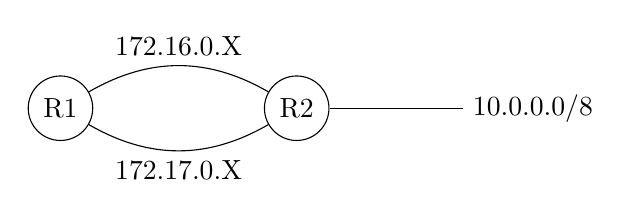
\begin{tikzpicture}[node distance=3cm]
			\node[circle,draw] (1)              {R1};
			\node[circle,draw] (2) [right of=1] {R2};
			\node              (3) [right of=2] {10.0.0.0/8};
			\path (1) edge [bend left]  node[above] {172.16.0.X} (2)
			          edge [bend right] node[below] {172.17.0.X} (2)
			      (2) edge                                       (3);
		\end{tikzpicture}
	\end{center}
	\texttt{\pause\\)\#ip route 10.0.0.0 255.0.0.0 172.16.0.2 10
	        \pause\\)\#ip route 10.0.0.0 255.0.0.0 172.17.0.2 20
	}
\end{frame}
